\documentclass[11pt,aspectratio=169]{beamer}
\usepackage[T1]{fontenc}
\usepackage[utf8]{inputenc}
\usepackage[english]{babel}
\usepackage{mathpazo}
\usefonttheme{serif}
\usepackage{amsmath,amssymb,booktabs,array,tabularx,graphicx,microtype}
\usepackage{adjustbox}
\usepackage{tikz}
\usetikzlibrary{arrows.meta,calc,positioning,decorations.pathreplacing,patterns,fit,backgrounds}

% Figures come from the idea folder; the TikZ figures in tikz/ are copies of those of the note.
\graphicspath{{../../../ideas/group-identification/figures/}}

% Colours of the note: i, j and a third flight; neutrals for text, grids and fills.
\definecolor{blueI}{HTML}{2A78D6}
\definecolor{orangeJ}{HTML}{EB6834}
\definecolor{aqua}{HTML}{1BAF7A}
\definecolor{ink}{HTML}{0B0B0B}
\definecolor{ink2}{HTML}{52514E}
\definecolor{muted}{HTML}{9A9893}
\definecolor{light}{HTML}{E6E5E1}
\definecolor{steel}{RGB}{74,96,121}
\definecolor{steellight}{RGB}{192,206,220}

\tikzset{
  >={Stealth[length=1.8mm]},
  every picture/.style={line cap=round, line join=round},
  lbl/.style={font=\footnotesize},
  note/.style={font=\footnotesize, text=ink2},
}

\newcommand{\x}{\mathbf{x}}
\newcommand{\M}{\mathcal{M}}
\newcommand{\dep}{\mathrm{dep}}
\newcommand{\FDR}{\widehat{\mathrm{FDR}}}

% Theme: steel-blue title bar, white pages, as in the earlier decks.
\setbeamercolor{structure}{fg=steel}
\setbeamercolor{normal text}{fg=ink,bg=white}
\setbeamercolor{frametitle}{fg=white,bg=steel}
\setbeamercolor{alerted text}{fg=blueI}
\setbeamercolor{takeaway}{fg=steel,bg=steellight!30}
\setbeamercolor{defbox}{fg=ink,bg=steellight!28}
\setbeamersize{text margin left=7mm,text margin right=7mm}
\setbeamertemplate{navigation symbols}{}
\setbeamertemplate{itemize item}{\textcolor{steel}{\small$\bullet$}}
\setbeamertemplate{itemize subitem}{\textcolor{steel}{\textendash}}
\setbeamertemplate{itemize/enumerate body begin}{\setlength{\itemsep}{0.3em}}
\setbeamertemplate{frametitle}{%
  \nointerlineskip
  \begin{beamercolorbox}[wd=\paperwidth,ht=9mm,dp=3mm,center]{frametitle}
    \large\insertframetitle\strut
  \end{beamercolorbox}
  \begin{tikzpicture}[remember picture,overlay]
    \node[anchor=north east,text=white,inner sep=0pt,xshift=-2.3mm,yshift=-4.2mm]
      at(current page.north east){\small\insertframenumber};
  \end{tikzpicture}}
\setbeamertemplate{footline}{%
  \hspace{7mm}\textcolor{muted}{\fontsize{6.5}{8}\selectfont
   October 2026}\vspace{2mm}}

\newcommand{\source}[1]{\par\vspace{1mm}{\fontsize{7}{8.3}\selectfont\color{ink2}#1\par}}
\newcommand{\takeaway}[1]{\par\vfill
  \begin{beamercolorbox}[wd=\linewidth,sep=5pt]{takeaway}\small #1\end{beamercolorbox}}
% A definition: its name in bold, then the statement, on a pale band.
\newcommand{\defn}[2]{%
  \begin{beamercolorbox}[wd=\linewidth,sep=5pt]{defbox}\small\textcolor{steel}{\textbf{#1.}}\enspace #2\end{beamercolorbox}}
% A TikZ figure of the note, scaled to fit the given height and the line width.
\newcommand{\tikzfig}[2][0.8\textheight]{%
  \begin{center}\adjustbox{max width=\linewidth,max height=#1}{\input{tikz/#2}}\end{center}}
% A figure of the note at full width, at most the given height.
\newcommand{\fig}[2][0.5\textheight]{%
  \begin{center}\includegraphics[width=\linewidth,height=#1,keepaspectratio]{#2}\end{center}}
% A full-page divider that opens one part of the talk.
\newcommand{\partframe}[2]{%
\begin{frame}[plain,noframenumbering]
\begin{tikzpicture}[remember picture,overlay]
 \fill[steel](current page.south west)rectangle(current page.north east);
 \node[text=white,align=center,text width=.82\paperwidth]at([yshift=4mm]current page.center)
   {{\Large\bfseries #1}\\[3mm]{\normalsize\color{steellight}#2}};
\end{tikzpicture}
\end{frame}}

\hypersetup{pdftitle={Method assessment},pdfauthor={Matteo Di Sante},
  colorlinks=true,urlcolor=blueI,linkcolor=blueI}

\begin{document}

\begin{frame}[plain]
\begin{tikzpicture}[remember picture,overlay]
 \fill[steel](current page.south west)rectangle(current page.north east);
 \fill[steellight](current page.south west)rectangle([yshift=20mm]current page.south east);
 \node[text=white,align=center,text width=.9\paperwidth]at([yshift=8mm]current page.center)
   {{\LARGE\bfseries The effect of chance on group identification}\\[4mm]
   {\small Group identificaiton}};
 \node[text=steel,align=center]at([yshift=10mm]current page.south)
   {{\normalsize October 2026}\\[1.5mm]};
\end{tikzpicture}
\end{frame}

\begin{frame}{The question}
\begin{itemize}
  \item Contact: close in space, at most $\delta$ apart in time.
  \item Same takeoff, ridges, thermals: chance contacts, mostly short.
  \item We keep contacts lasting $\ge\tau^*$.
\end{itemize}
\tikzfig[0.32\textheight]{contacts}
\begin{beamercolorbox}[wd=\linewidth,sep=6pt,center]{takeaway}
\large Can a null model that counts the chance contacts give $\tau^*$?
\end{beamercolorbox}
\source{162\,485 flights, 6\,209 dates, FFVL archive; profiles on 300 dates.}
\end{frame}

\partframe{Part 1: Null model, false discovery rate, $\tau^*$}{}

\begin{frame}{Null model: shift one flight in time}
\defn{Surrogate pair}{$i,j$ same date, $\|\x_i(k^0_i)-\x_j(k^0_j)\|<R_s=10$~km:
\[
  \x^s_j(t)=\x_j(t+r),\qquad r=(k^0_j-k^0_i)-\vartheta,\qquad
  \vartheta\sim\hat P\bigl(k^0_j-k^0_i\bigr),\qquad |r|\ge2\delta+\Delta
\]}
\tikzfig[0.3\textheight]{null}
\[
  (t,t')\in\M_{ij}\ \Rightarrow\ |t-(t'-r)|\ge|r|-\delta>\delta
\]
\source{Keeps route, terrain, date; destroys every real correspondence. Spiegel et al.\ (2016).}
\end{frame}

\begin{frame}{Shifts of about an hour}
\begin{columns}[c,onlytextwidth]
\column{.55\textwidth}
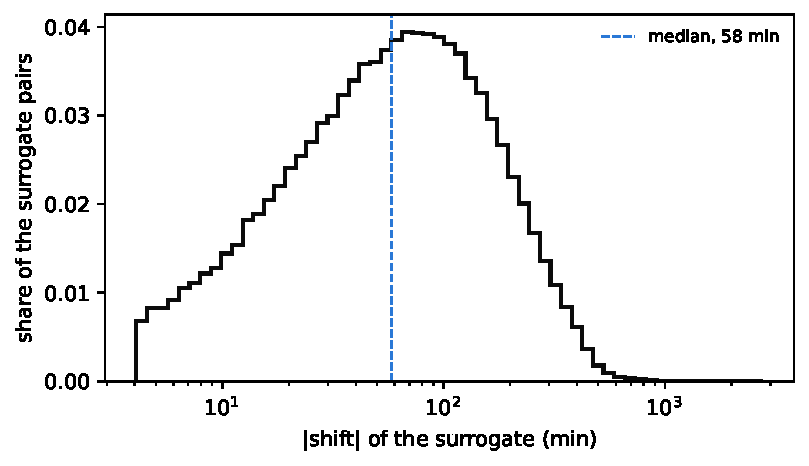
\includegraphics[width=\linewidth]{assessment_shifts.pdf}
\column{.42\textwidth}
\[
  \mathrm{median}\,|r|=58~\text{min}
\]
\[
  |r|\in[8~\text{min},\,4.4~\text{h}]\quad(90\%)
\]
\par\medskip
\centering\small $\Rightarrow$ the copy flies in the weather of another hour
\end{columns}
\source{248\,741 surrogate pairs, whole archive.}
\end{frame}

\begin{frame}{False discovery rate}
\defn{Definitions}{\begin{itemize}\setlength{\itemsep}{0pt}
  \item $M_d(\tau)$: surrogate intervals $\ge\tau$ on date $d$
  \item $S_d$, $H_d$: surrogate and real exposure on date $d$ (time both fly)
  \item $N(\tau)$: real intervals $\ge\tau$, all dates
\end{itemize}}
\[
  \rho_{0,d}(\tau)=\frac{M_d(\tau)}{S_d},\qquad
  C(\tau)=\sum_d\rho_{0,d}(\tau)\,H_d
\]
\[
  \FDR(\tau)=\frac{C(\tau)}{N(\tau)},\qquad
  \tau^*=\min\bigl\{\tau:\ \FDR(\tau)\le q\bigr\}
\]
\source{SAM (Tusher et al.\ 2001), with time shifts in place of permutations.}
\end{frame}

\begin{frame}{Most short contacts are chance}
\fig[0.48\textheight]{assessment_fdr.pdf}
\[
  \FDR(0)=0.74,\qquad \FDR(10~\text{min})=0.47,\qquad \FDR(30~\text{min})=0.16
\]
\[
  q=0.1\ \Rightarrow\ \tau^*=38.1~\text{min}
\]
\source{$\delta=2$~min (blue), 5~min (grey). Bracket: 5--95\% over 200 resamplings of the dates.}
\end{frame}

\begin{frame}{How much the shift matters}
\begin{center}
\begin{tabular}{@{}l c c c@{}}
\toprule
surrogates & $\FDR(10~\text{min})$ & $\FDR(30~\text{min})$ & $\tau^*$ (min) \\
\midrule
all $|r|$ & 0.48 & 0.16 & 38.2 \\
$|r|<30$ min & 0.73 & 0.31 & 53.3 \\
$|r|\ge60$ min & 0.26 & 0.05 & 23.0 \\
\bottomrule
\end{tabular}
\end{center}
\[
  \tau^*\in[23,\,53]~\text{min, set by}\ |r|
\]
\defn{Why $\tau^*$ is longer for short $|r|$}{A real follower of $i$ more than $\delta$ behind is
no contact in the real data. A short shift brings it within $\delta$: it counts as chance, though
it is a real pair.}
\medskip
\defn{Why $\tau^*$ is shorter for long $|r|$}{Two real pilots of the same hour both go where the thermals
work, so they meet without flying together. The copy of $j$ flies in another hour's weather and
does not go where $i$ is. These chance meetings are in the real data but not in the surrogates: chance
is underestimated.}
\source{$q=0.1$, $\delta=2$~min, 2\,737 dates with all classes. We keep $r$ from the takeoff
delays.}
\end{frame}

\partframe{Part 2: parameters}{Measured, chosen, or definitions}

\begin{frame}{Three kinds of parameters}
\begin{center}
\begin{tabular}{@{}l l l@{}}
\toprule
& value & set by \\
\midrule
$\delta$ & 2 min & chosen/measured: $R(l)$ \\
$q$ & 0.1 & chosen/measured \\
$\tau^*$ & 38.1 min & $\FDR(\tau^*)\le q$ \\
$\varepsilon_h$, $\varepsilon_z$, $g$ & 500 m, 300 m, 120 s & chosen \\
$\theta_{\max}$ & 45$^\circ$ & no effect \\
$\Delta$, $h_{\max}$, $R_\dep$, $v_{\max}$, $R_s$, $r_{\min}$ & & fixed: bounds, exactness \\
\bottomrule
\end{tabular}
\end{center}
\end{frame}

\begin{frame}{$\delta$: delay profile}
\[
  R(l)=\frac{n_{\rm real}(l)/H_{\rm real}}{n_{\rm chance}(l)/H_{\rm chance}},\qquad
  n(l)=\#\{(t,t+l)\in\M\}
\]
\fig[0.4\textheight]{assessment_delays.pdf}
\[
  R_{\max}=5.6,\quad R(105~\text{s})\approx4,\quad R(195~\text{s})\approx3,\quad
  R(500~\text{s})\approx2,\quad R(15~\text{min})=1.5
\]
\source{300 dates, window 15~min. Fast part: flying together; slow tail: same thermals, same hour.}
\end{frame}

\begin{frame}{$\delta$: long contacts, short delays}
\[
  \ell_{\rm med}=\mathrm{median}\bigl\{l^*(t):\ t\in[t_{\rm on},t_{\rm off}),\ \text{no search}\bigr\}
\]
\begin{center}
\small
\begin{tabular}{@{}l c c c@{}}
\toprule
duration & median $|\ell_{\rm med}|$ & $|\ell_{\rm med}|\le2$ min & $|\ell_{\rm med}|\ge285$ s \\
\midrule
$<10$ min & 210 s & 32\% & 29\% \\
10--30 min & 160 s & 39\% & 12\% \\
30--90 min & 80 s & 64\% & 2.1\% \\
$\ge90$ min & 25 s & 90\% & 6 of 10\,734 \\
\bottomrule
\end{tabular}
\end{center}
\[
  \delta=2~\text{min}:\qquad R(\delta)=3.7,\qquad
  P\bigl(|\ell_{\rm med}|\le\delta\ \big|\ \text{duration}\ge90~\text{min}\bigr)=0.9
\]
\source{Run with $\delta=5$~min, 965\,770 intervals.}
\end{frame}

\begin{frame}{Distance at the same instant}
\[
  g(d)=\frac{p_{\rm real}(d)}{p_{\rm chance}(d)},\qquad d=\|\x_i(t)-\x_j(t)\|
\]
\fig[0.4\textheight]{assessment_separation.pdf}
\[
  g(d<100~\text{m})=10.4,\quad g<1\ \text{for}\ d>5.7~\text{km},\quad
  \text{in contact: } d\le\varepsilon_h+v_{\max}\delta\approx3.8~\text{km}
\]
\source{210 dates, every instant both fly. Excess beyond sight (1.5~km): weather of the hour too.}
\end{frame}

\begin{frame}{Tolerances: no edge}
\[
  d_h(t)=\min_{|l|\le\delta,\ |\Delta z_l|<\varepsilon_z}\|\Delta\x_l\|,\qquad
  d_z(t)=\min_{|l|\le\delta,\ \|\Delta\x_l\|<\varepsilon_h}|\Delta z_l|
\]
\fig[0.4\textheight]{assessment_tolerances.pdf}
\[
  \frac{\text{real}}{\text{chance}}\approx1.5\ \text{at}\ \varepsilon_h,\ \varepsilon_z;\qquad
  \text{gaps: same lengths}\ \Rightarrow\ \varepsilon_h,\varepsilon_z,g\ \text{definitions}
\]
\source{$\Delta\x_l=\x_i(t)-\x_j(t+l)$, $\Delta z_l=z_i(t)-z_j(t+l)$; 210 dates, $\delta=2$~min.}
\end{frame}


\begin{frame}{$q$: how much chance we accept}
\fig[0.38\textheight]{assessment_q.pdf}
\begin{center}
\small
\begin{tabular}{@{}c c c c c@{}}
\toprule
$q$ & $\tau^*$ (min) & para in a group & hang in a group & episodes \\
\midrule
0.05 & 51.9 & 13.7\% & 3.8\% & 10\,553 \\
0.1 & 38.1 & 21.7\% & 6.9\% & 17\,169 \\
0.2 & 26.4 & 31.7\% & 13.9\% & 26\,504 \\
\bottomrule
\end{tabular}
\end{center}
\source{$\delta=2$~min. We take $q=0.1$.}
\end{frame}




\begin{frame}{In short}
\[
  \text{chance:}\quad \x_j(t)\to\x_j(t+r),\quad |r|\sim1~\text{h}
\]
\[
  \FDR(\tau^*)\le0.1\ \Rightarrow\ \tau^*=38.1~\text{min}
\]
\[
  \delta=2~\text{min}:\quad \text{real/chance}(\delta)=R(\delta)=3.7,\quad 90\%\ \text{of long contacts}
\]
\[
  \varepsilon_h,\ \varepsilon_z,\ g:\ \text{definitions}
\]
\takeaway{In a group at some point: 21.7\% of the paraglider flights, 6.9\% of the hang-glider
flights; 17\,169 episodes.}
\end{frame}

\end{document}
